\documentclass[a4paper]{article}

\def\npart{III}
\def\nterm {Lent}
\def\nyear {2017-2018}
\def\nlecturer {Brian}
\def\ncourse {Angular JS}

\makeatletter
\ifx \nauthor\undefined
  \def\nauthor{Dexter Chua}
\else
\fi

\author{Based on lectures by \nlecturer \\\small Notes taken by \nauthor}
\date{\nterm\ \nyear}

\usepackage{alltt}
\usepackage{amsfonts}
\usepackage{amsmath}
\usepackage{amssymb}
\usepackage{amsthm}
\usepackage{booktabs}
\usepackage{caption}
\usepackage{enumitem}
\usepackage{fancyhdr}
\usepackage{graphicx}
\usepackage{mathdots}
\usepackage{mathtools}
\usepackage{microtype}
\usepackage{multirow}
\usepackage{pdflscape}
\usepackage{pgfplots}
\usepackage{siunitx}
\usepackage{slashed}
\usepackage{tabularx}
\usepackage{tikz}
\usepackage{tkz-euclide}
\usepackage[normalem]{ulem}
\usepackage[all]{xy}
\usepackage{imakeidx}



\makeindex[intoc, title=Index]
\indexsetup{othercode={\lhead{\emph{Index}}}}

\ifx \nextra \undefined
  \usepackage[pdftex,
    hidelinks,
    pdfauthor={Dexter Chua},
    pdfsubject={Cambridge Maths Notes: Part \npart\ - \ncourse},
    pdftitle={Part \npart\ - \ncourse},
  pdfkeywords={Cambridge Mathematics Maths Math \npart\ \nterm\ \nyear\ \ncourse}]{hyperref}
  \title{Part \npart\ --- \ncourse}
\else
  \usepackage[pdftex,
    hidelinks,
    pdfauthor={Dexter Chua},
    pdfsubject={Cambridge Maths Notes: Part \npart\ - \ncourse\ (\nextra)},
    pdftitle={Part \npart\ - \ncourse\ (\nextra)},
  pdfkeywords={Cambridge Mathematics Maths Math \npart\ \nterm\ \nyear\ \ncourse\ \nextra}]{hyperref}

  \title{Part \npart\ --- \ncourse \\ {\Large \nextra}}
  \renewcommand\printindex{}
\fi

\pgfplotsset{compat=1.12}

\pagestyle{fancyplain}
\ifx \ncoursehead \undefined
\def\ncoursehead{\ncourse}
\fi

\lhead{\emph{\nouppercase{\leftmark}}}
\ifx \nextra \undefined
  \rhead{
    \ifnum\thepage=1
    \else
      \npart\ \ncoursehead
    \fi}
\else
  \rhead{
    \ifnum\thepage=1
    \else
      \npart\ \ncoursehead \ (\nextra)
    \fi}
\fi
\usetikzlibrary{arrows.meta}
\usetikzlibrary{decorations.markings}
\usetikzlibrary{decorations.pathmorphing}
\usetikzlibrary{positioning}
\usetikzlibrary{fadings}
\usetikzlibrary{intersections}
\usetikzlibrary{cd}

\newcommand*{\Cdot}{{\raisebox{-0.25ex}{\scalebox{1.5}{$\cdot$}}}}
\newcommand {\pd}[2][ ]{
  \ifx #1 { }
    \frac{\partial}{\partial #2}
  \else
    \frac{\partial^{#1}}{\partial #2^{#1}}
  \fi
}
\ifx \nhtml \undefined
\else
  \renewcommand\printindex{}
  \DisableLigatures[f]{family = *}
  \let\Contentsline\contentsline
  \renewcommand\contentsline[3]{\Contentsline{#1}{#2}{}}
  \renewcommand{\@dotsep}{10000}
  \newlength\currentparindent
  \setlength\currentparindent\parindent

  \newcommand\@minipagerestore{\setlength{\parindent}{\currentparindent}}
  \usepackage[active,tightpage,pdftex]{preview}
  \renewcommand{\PreviewBorder}{0.1cm}

  \newenvironment{stretchpage}%
  {\begin{preview}\begin{minipage}{\hsize}}%
    {\end{minipage}\end{preview}}
  \AtBeginDocument{\begin{stretchpage}}
  \AtEndDocument{\end{stretchpage}}

  \newcommand{\@@newpage}{\end{stretchpage}\begin{stretchpage}}

  \let\@real@section\section
  \renewcommand{\section}{\@@newpage\@real@section}
  \let\@real@subsection\subsection
  \renewcommand{\subsection}{\@ifstar{\@real@subsection*}{\@@newpage\@real@subsection}}
\fi
\ifx \ntrim \undefined
\else
  \usepackage{geometry}
  \geometry{
    papersize={379pt, 699pt},
    textwidth=345pt,
    textheight=596pt,
    left=17pt,
    top=54pt,
    right=17pt
  }
\fi

\ifx \nisofficial \undefined
\let\@real@maketitle\maketitle
\renewcommand{\maketitle}{\@real@maketitle\begin{center}\begin{minipage}[c]{0.9\textwidth}\centering\footnotesize These notes are not endorsed by the lecturers, and I have modified them (often significantly) after lectures. They are nowhere near accurate representations of what was actually lectured, and in particular, all errors are almost surely mine.\end{minipage}\end{center}}
\else
\fi

% Theorems
\theoremstyle{definition}
\newtheorem*{aim}{Aim}
\newtheorem*{axiom}{Axiom}
\newtheorem*{claim}{Claim}
\newtheorem*{cor}{Corollary}
\newtheorem*{conjecture}{Conjecture}
\newtheorem*{defi}{Definition}
\newtheorem*{eg}{Example}
\newtheorem*{ex}{Exercise}
\newtheorem*{fact}{Fact}
\newtheorem*{law}{Law}
\newtheorem*{lemma}{Lemma}
\newtheorem*{notation}{Notation}
\newtheorem*{prop}{Proposition}
\newtheorem*{question}{Question}
\newtheorem*{rrule}{Rule}
\newtheorem*{thm}{Theorem}
\newtheorem*{assumption}{Assumption}

\newtheorem*{remark}{Remark}
\newtheorem*{warning}{Warning}
\newtheorem*{exercise}{Exercise}

\newtheorem{nthm}{Theorem}[section]
\newtheorem{nlemma}[nthm]{Lemma}
\newtheorem{nprop}[nthm]{Proposition}
\newtheorem{ncor}[nthm]{Corollary}


\renewcommand{\labelitemi}{--}
\renewcommand{\labelitemii}{$\circ$}
\renewcommand{\labelenumi}{(\roman{*})}

\let\stdsection\section
\renewcommand\section{\newpage\stdsection}

\newcommand\qedsym{\hfill\ensuremath{\square}}
% Strike through
\def\st{\bgroup \ULdepth=-.55ex \ULset}


%%%%%%%%%%%%%%%%%%%%%%%%%
%%%%% Maths Symbols %%%%%
%%%%%%%%%%%%%%%%%%%%%%%%%

% Matrix groups
\newcommand{\GL}{\mathrm{GL}}
\newcommand{\Or}{\mathrm{O}}
\newcommand{\PGL}{\mathrm{PGL}}
\newcommand{\PSL}{\mathrm{PSL}}
\newcommand{\PSO}{\mathrm{PSO}}
\newcommand{\PSU}{\mathrm{PSU}}
\newcommand{\SL}{\mathrm{SL}}
\newcommand{\SO}{\mathrm{SO}}
\newcommand{\Spin}{\mathrm{Spin}}
\newcommand{\Sp}{\mathrm{Sp}}
\newcommand{\SU}{\mathrm{SU}}
\newcommand{\U}{\mathrm{U}}
\newcommand{\Mat}{\mathrm{Mat}}

% Matrix algebras
\newcommand{\gl}{\mathfrak{gl}}
\newcommand{\ort}{\mathfrak{o}}
\newcommand{\so}{\mathfrak{so}}
\newcommand{\su}{\mathfrak{su}}
\newcommand{\uu}{\mathfrak{u}}
\renewcommand{\sl}{\mathfrak{sl}}

% Special sets
\newcommand{\C}{\mathbb{C}}
\newcommand{\CP}{\mathbb{CP}}
\newcommand{\GG}{\mathbb{G}}
\newcommand{\N}{\mathbb{N}}
\newcommand{\Q}{\mathbb{Q}}
\newcommand{\R}{\mathbb{R}}
\newcommand{\RP}{\mathbb{RP}}
\newcommand{\T}{\mathbb{T}}
\newcommand{\Z}{\mathbb{Z}}
\renewcommand{\H}{\mathbb{H}}

% Brackets
\newcommand{\abs}[1]{\left\lvert #1\right\rvert}
\newcommand{\bket}[1]{\left\lvert #1\right\rangle}
\newcommand{\brak}[1]{\left\langle #1 \right\rvert}
\newcommand{\braket}[2]{\left\langle #1\middle\vert #2 \right\rangle}
\newcommand{\bra}{\langle}
\newcommand{\ket}{\rangle}
\newcommand{\norm}[1]{\left\lVert #1\right\rVert}
\newcommand{\normalorder}[1]{\mathop{:}\nolimits\!#1\!\mathop{:}\nolimits}
\newcommand{\tv}[1]{|#1|}
\renewcommand{\vec}[1]{\boldsymbol{\mathbf{#1}}}

% not-math
\newcommand{\bolds}[1]{{\bfseries #1}}
\newcommand{\cat}[1]{\mathsf{#1}}
\newcommand{\ph}{\,\cdot\,}
\newcommand{\term}[1]{\emph{#1}\index{#1}}
\newcommand{\phantomeq}{\hphantom{{}={}}}
% Probability
\DeclareMathOperator{\Bernoulli}{Bernoulli}
\DeclareMathOperator{\betaD}{beta}
\DeclareMathOperator{\bias}{bias}
\DeclareMathOperator{\binomial}{binomial}
\DeclareMathOperator{\corr}{corr}
\DeclareMathOperator{\cov}{cov}
\DeclareMathOperator{\gammaD}{gamma}
\DeclareMathOperator{\mse}{mse}
\DeclareMathOperator{\multinomial}{multinomial}
\DeclareMathOperator{\Poisson}{Poisson}
\DeclareMathOperator{\var}{var}
\newcommand{\E}{\mathbb{E}}
\newcommand{\Prob}{\mathbb{P}}

% Algebra
\DeclareMathOperator{\adj}{adj}
\DeclareMathOperator{\Ann}{Ann}
\DeclareMathOperator{\Aut}{Aut}
\DeclareMathOperator{\Char}{char}
\DeclareMathOperator{\disc}{disc}
\DeclareMathOperator{\dom}{dom}
\DeclareMathOperator{\fix}{fix}
\DeclareMathOperator{\Hom}{Hom}
\DeclareMathOperator{\id}{id}
\DeclareMathOperator{\image}{image}
\DeclareMathOperator{\im}{im}
\DeclareMathOperator{\tr}{tr}
\DeclareMathOperator{\Tr}{Tr}
\newcommand{\Bilin}{\mathrm{Bilin}}
\newcommand{\Frob}{\mathrm{Frob}}

% Others
\newcommand\ad{\mathrm{ad}}
\newcommand\Art{\mathrm{Art}}
\newcommand{\B}{\mathcal{B}}
\newcommand{\cU}{\mathcal{U}}
\newcommand{\Der}{\mathrm{Der}}
\newcommand{\D}{\mathrm{D}}
\newcommand{\dR}{\mathrm{dR}}
\newcommand{\exterior}{\mathchoice{{\textstyle\bigwedge}}{{\bigwedge}}{{\textstyle\wedge}}{{\scriptstyle\wedge}}}
\newcommand{\F}{\mathbb{F}}
\newcommand{\G}{\mathcal{G}}
\newcommand{\Gr}{\mathrm{Gr}}
\newcommand{\haut}{\mathrm{ht}}
\newcommand{\Hol}{\mathrm{Hol}}
\newcommand{\hol}{\mathfrak{hol}}
\newcommand{\Id}{\mathrm{Id}}
\newcommand{\lie}[1]{\mathfrak{#1}}
\newcommand{\op}{\mathrm{op}}
\newcommand{\Oc}{\mathcal{O}}
\newcommand{\pr}{\mathrm{pr}}
\newcommand{\Ps}{\mathcal{P}}
\newcommand{\pt}{\mathrm{pt}}
\newcommand{\qeq}{\mathrel{``{=}"}}
\newcommand{\Rs}{\mathcal{R}}
\newcommand{\Vect}{\mathrm{Vect}}
\newcommand{\wsto}{\stackrel{\mathrm{w}^*}{\to}}
\newcommand{\wt}{\mathrm{wt}}
\newcommand{\wto}{\stackrel{\mathrm{w}}{\to}}
\renewcommand{\d}{\mathrm{d}}
\renewcommand{\P}{\mathbb{P}}
%\renewcommand{\F}{\mathcal{F}}


\let\Im\relax
\let\Re\relax

\DeclareMathOperator{\area}{area}
\DeclareMathOperator{\card}{card}
\DeclareMathOperator{\ccl}{ccl}
\DeclareMathOperator{\ch}{ch}
\DeclareMathOperator{\cl}{cl}
\DeclareMathOperator{\cls}{\overline{\mathrm{span}}}
\DeclareMathOperator{\coker}{coker}
\DeclareMathOperator{\conv}{conv}
\DeclareMathOperator{\cosec}{cosec}
\DeclareMathOperator{\cosech}{cosech}
\DeclareMathOperator{\covol}{covol}
\DeclareMathOperator{\diag}{diag}
\DeclareMathOperator{\diam}{diam}
\DeclareMathOperator{\Diff}{Diff}
\DeclareMathOperator{\End}{End}
\DeclareMathOperator{\energy}{energy}
\DeclareMathOperator{\erfc}{erfc}
\DeclareMathOperator{\erf}{erf}
\DeclareMathOperator*{\esssup}{ess\,sup}
\DeclareMathOperator{\ev}{ev}
\DeclareMathOperator{\Ext}{Ext}
\DeclareMathOperator{\fst}{fst}
\DeclareMathOperator{\Fit}{Fit}
\DeclareMathOperator{\Frac}{Frac}
\DeclareMathOperator{\Gal}{Gal}
\DeclareMathOperator{\gr}{gr}
\DeclareMathOperator{\hcf}{hcf}
\DeclareMathOperator{\Im}{Im}
\DeclareMathOperator{\Ind}{Ind}
\DeclareMathOperator{\Int}{Int}
\DeclareMathOperator{\Isom}{Isom}
\DeclareMathOperator{\lcm}{lcm}
\DeclareMathOperator{\length}{length}
\DeclareMathOperator{\Lie}{Lie}
\DeclareMathOperator{\like}{like}
\DeclareMathOperator{\Lk}{Lk}
\DeclareMathOperator{\Maps}{Maps}
\DeclareMathOperator{\orb}{orb}
\DeclareMathOperator{\ord}{ord}
\DeclareMathOperator{\otp}{otp}
\DeclareMathOperator{\poly}{poly}
\DeclareMathOperator{\rank}{rank}
\DeclareMathOperator{\rel}{rel}
\DeclareMathOperator{\Rad}{Rad}
\DeclareMathOperator{\Re}{Re}
\DeclareMathOperator*{\res}{res}
\DeclareMathOperator{\Res}{Res}
\DeclareMathOperator{\Ric}{Ric}
\DeclareMathOperator{\rk}{rk}
\DeclareMathOperator{\Rees}{Rees}
\DeclareMathOperator{\Root}{Root}
\DeclareMathOperator{\sech}{sech}
\DeclareMathOperator{\sgn}{sgn}
\DeclareMathOperator{\snd}{snd}
\DeclareMathOperator{\Spec}{Spec}
\DeclareMathOperator{\spn}{span}
\DeclareMathOperator{\stab}{stab}
\DeclareMathOperator{\St}{St}
\DeclareMathOperator{\supp}{supp}
\DeclareMathOperator{\Syl}{Syl}
\DeclareMathOperator{\Sym}{Sym}
\DeclareMathOperator{\vol}{vol}

\pgfarrowsdeclarecombine{twolatex'}{twolatex'}{latex'}{latex'}{latex'}{latex'}
\tikzset{->/.style = {decoration={markings,
                                  mark=at position 1 with {\arrow[scale=2]{latex'}}},
                      postaction={decorate}}}
\tikzset{<-/.style = {decoration={markings,
                                  mark=at position 0 with {\arrowreversed[scale=2]{latex'}}},
                      postaction={decorate}}}
\tikzset{<->/.style = {decoration={markings,
                                   mark=at position 0 with {\arrowreversed[scale=2]{latex'}},
                                   mark=at position 1 with {\arrow[scale=2]{latex'}}},
                       postaction={decorate}}}
\tikzset{->-/.style = {decoration={markings,
                                   mark=at position #1 with {\arrow[scale=2]{latex'}}},
                       postaction={decorate}}}
\tikzset{-<-/.style = {decoration={markings,
                                   mark=at position #1 with {\arrowreversed[scale=2]{latex'}}},
                       postaction={decorate}}}
\tikzset{->>/.style = {decoration={markings,
                                  mark=at position 1 with {\arrow[scale=2]{latex'}}},
                      postaction={decorate}}}
\tikzset{<<-/.style = {decoration={markings,
                                  mark=at position 0 with {\arrowreversed[scale=2]{twolatex'}}},
                      postaction={decorate}}}
\tikzset{<<->>/.style = {decoration={markings,
                                   mark=at position 0 with {\arrowreversed[scale=2]{twolatex'}},
                                   mark=at position 1 with {\arrow[scale=2]{twolatex'}}},
                       postaction={decorate}}}
\tikzset{->>-/.style = {decoration={markings,
                                   mark=at position #1 with {\arrow[scale=2]{twolatex'}}},
                       postaction={decorate}}}
\tikzset{-<<-/.style = {decoration={markings,
                                   mark=at position #1 with {\arrowreversed[scale=2]{twolatex'}}},
                       postaction={decorate}}}

\tikzset{circ/.style = {fill, circle, inner sep = 0, minimum size = 3}}
\tikzset{scirc/.style = {fill, circle, inner sep = 0, minimum size = 1.5}}
\tikzset{mstate/.style={circle, draw, blue, text=black, minimum width=0.7cm}}

\tikzset{eqpic/.style={baseline={([yshift=-.5ex]current bounding box.center)}}}
\tikzset{commutative diagrams/.cd,cdmap/.style={/tikz/column 1/.append style={anchor=base east},/tikz/column 2/.append style={anchor=base west},row sep=tiny}}

\definecolor{mblue}{rgb}{0.2, 0.3, 0.8}
\definecolor{morange}{rgb}{1, 0.5, 0}
\definecolor{mgreen}{rgb}{0.1, 0.4, 0.2}
\definecolor{mred}{rgb}{0.5, 0, 0}

\def\drawcirculararc(#1,#2)(#3,#4)(#5,#6){%
    \pgfmathsetmacro\cA{(#1*#1+#2*#2-#3*#3-#4*#4)/2}%
    \pgfmathsetmacro\cB{(#1*#1+#2*#2-#5*#5-#6*#6)/2}%
    \pgfmathsetmacro\cy{(\cB*(#1-#3)-\cA*(#1-#5))/%
                        ((#2-#6)*(#1-#3)-(#2-#4)*(#1-#5))}%
    \pgfmathsetmacro\cx{(\cA-\cy*(#2-#4))/(#1-#3)}%
    \pgfmathsetmacro\cr{sqrt((#1-\cx)*(#1-\cx)+(#2-\cy)*(#2-\cy))}%
    \pgfmathsetmacro\cA{atan2(#2-\cy,#1-\cx)}%
    \pgfmathsetmacro\cB{atan2(#6-\cy,#5-\cx)}%
    \pgfmathparse{\cB<\cA}%
    \ifnum\pgfmathresult=1
        \pgfmathsetmacro\cB{\cB+360}%
    \fi
    \draw (#1,#2) arc (\cA:\cB:\cr);%
}
\newcommand\getCoord[3]{\newdimen{#1}\newdimen{#2}\pgfextractx{#1}{\pgfpointanchor{#3}{center}}\pgfextracty{#2}{\pgfpointanchor{#3}{center}}}

\newcommand\qedshift{\vspace{-17pt}}
\newcommand\fakeqed{\pushQED{\qed}\qedhere}

\def\Xint#1{\mathchoice
   {\XXint\displaystyle\textstyle{#1}}%
   {\XXint\textstyle\scriptstyle{#1}}%
   {\XXint\scriptstyle\scriptscriptstyle{#1}}%
   {\XXint\scriptscriptstyle\scriptscriptstyle{#1}}%
   \!\int}
\def\XXint#1#2#3{{\setbox0=\hbox{$#1{#2#3}{\int}$}
     \vcenter{\hbox{$#2#3$}}\kern-.5\wd0}}
\def\ddashint{\Xint=}
\def\dashint{\Xint-}

\newcommand\separator{{\centering\rule{2cm}{0.2pt}\vspace{2pt}\par}}

\newenvironment{own}{\color{gray!70!black}}{}

\newcommand\makecenter[1]{\raisebox{-0.5\height}{#1}}

\mathchardef\mdash="2D

\newenvironment{significant}{\begin{center}\begin{minipage}{0.9\textwidth}\centering\em}{\end{minipage}\end{center}}
\DeclareRobustCommand{\rvdots}{%
  \vbox{
    \baselineskip4\p@\lineskiplimit\z@
    \kern-\p@
    \hbox{.}\hbox{.}\hbox{.}
  }}
\DeclareRobustCommand\tph[3]{{\texorpdfstring{#1}{#2}}}
\makeatother


\usepackage{listings}
\usepackage{color}
\definecolor{lightgray}{rgb}{.9,.9,.9}
\definecolor{darkgray}{rgb}{.4,.4,.4}
\definecolor{purple}{rgb}{0.65, 0.12, 0.82}

\lstdefinelanguage{JavaScript}{
  keywords={typeof, new, true, false, catch, function, return, null, catch, switch, var, if, in, while, do, else, case, break},
  keywordstyle=\color{blue}\bfseries,
  ndkeywords={class, export, boolean, throw, implements, import, this},
  ndkeywordstyle=\color{darkgray}\bfseries,
  identifierstyle=\color{black},
  sensitive=false,
  comment=[l]{//},
  morecomment=[s]{/*}{*/},
  commentstyle=\color{purple}\ttfamily,
  stringstyle=\color{red}\ttfamily,
  morestring=[b]',
  morestring=[b]"
}

\lstset{
   language=JavaScript,
   backgroundcolor=\color{lightgray},
   extendedchars=true,
   basicstyle=\footnotesize\ttfamily,
   showstringspaces=false,
   showspaces=false,
   tabsize=2,
   breaklines=true,
   showtabs=false,
   captionpos=b
}

\setcounter{tocdepth}{2}

\begin{document}

\maketitle


\tableofcontents

\section{Introduction to Angular}
\subsection{Introduction}
Angular is an open source JavaScript framework maintained by Google. We use Angular to create single page applications (SPA).
\subsubsection{Single Page Application}

SPA are web applications that work like a desktop application. That means upon first loading the application the user downloads all the JavaScript, HTML and CSS to render any part of the application. Any extra data needed will be fetched dynamically when the user is using the application. However a total refresh is not necessary upon most circumstances.\\

We can summarize the difference between a SPA and a normal website as follow: normal website reloads on every click. SPA loads most HTML/CSS from the beginning and loads the necessary JSON while needed.\\

Therefore , you can regard the applications you created before as Multiple page applications. The application we can create with Angular is thus the contrary, Single Page Application.\\

Here is a diagram from Microsoft Documentation that summarize the difference pretty well

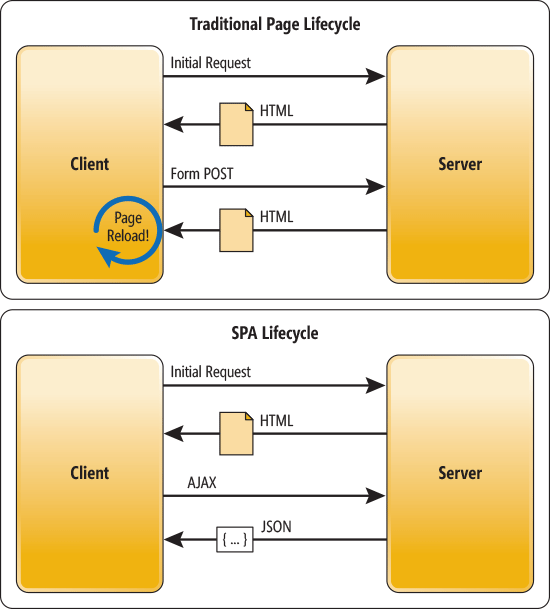
\includegraphics[scale = 0.5]{img/spa_vs_mpa.png}

The rendering of SPA and MPA also differs. Here is a diagram showing the difference in the rendering process.\\

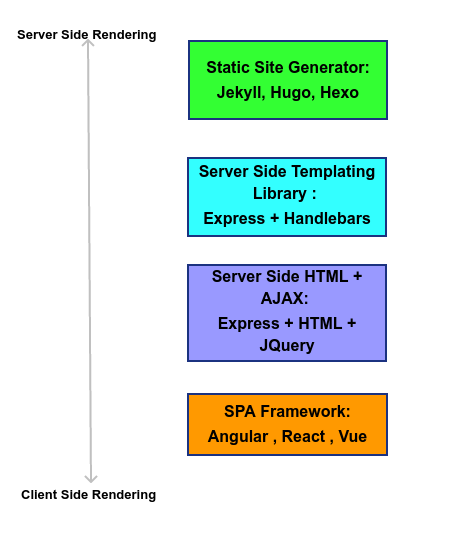
\includegraphics{img/rendering.png}

\subsubsection{Gmail}
One of the prominent example of a SPA is gmail. You have one page, which in its basic structure always looks the same. We can dynamically load any email but the basic structure doesn’t change just like many desktop applications (like MS Office). This set the standard for modern web development. Almost all the big websites these days makes use of SPA. Just take a good look at YouTube or Facebook.\\

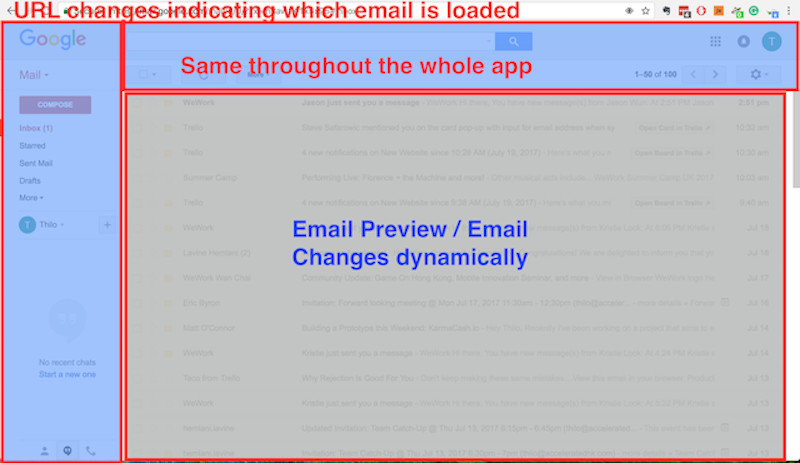
\includegraphics{img/spa.png}\\

\subsubsection{Different types of SPA Franework}

\subsubsection{MVVM vs MVS}
You may have heard the following two architectures. Model-View-Controller which specifies the three components in the architectures Model, View and Controller.\\

Here is the architecture for Model-View-Controller\\

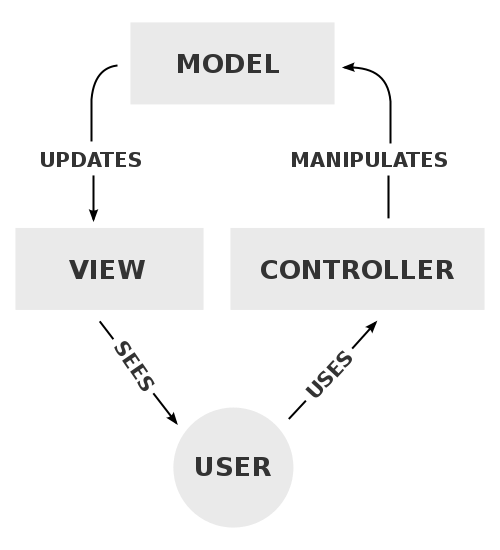
\includegraphics[scale = 0.5]{img/mvc.png}

In MVC, the users interacts with the controller which manipulates the model which is the data. The data is updated to view at the end.\\

Here is the architecture for Model-View-ViewModel\\

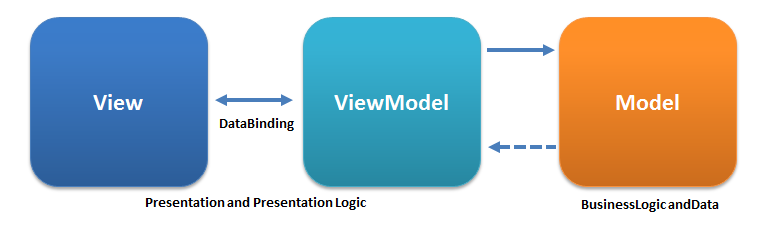
\includegraphics[scale = 0.5]{img/mvvm.png}

The biggest difference between MVVM and MVC lies in the reliance of Data Binding in MVVM. The data in ViewModel is bound to the view by the framework instead of updating through templates as in MVC.\\

For their application domains, nowadays MVC is mostly used in backend framework while MVVM is widely used in frontend framework.


\subsection{Installation}
The best way to create a new Angular project is through the Angular cli. So let’s do exactly that.\\

To install the cli run:
\begin{lstlisting}
npm install -g @angular/cli
\end{lstlisting}
Afterwards navigate to the folder where you save your coding projects. There we run:
\begin{lstlisting}
ng new sample-app
\end{lstlisting}
As you probably figured out yourself ng is short for angular. new creates a new project and sample-app is the project name. You’ll see in the terminal that angular creates a whole bunch of files and then installs a few things.\\

This is exactly the reason why we use the cli. Otherwise we would have to create those files manually and set up everything by ourselves, which would keep us pretty busy for a few hours (especially if we have no idea what we are doing).\\

Once that has finished let’s go check out our app.
\begin{lstlisting}
cd sample-app
ng serve
\end{lstlisting}
ng serve tells the cli to compile all the files and create a development server to serve the files from. Compiling in this process means that the Angular cli takes all the JavaScript files (our App will consist of many JS files) and bundles them together in a correct order. It will also make sure that our JS is readable by older browsers by changing it back to ES5 standards. These files are then served via a development server, the only thing special about this server is that we don’t have to set it up ourselves and that it recompiles automatically every time we change something in our code.\\

So let’s check out the project, go to http://localhost:4200\\

There you go your first Angular app up and running.

\subsubsection{Special for Bash on Ubuntu}
If you encounter error while you are installing angular cli through Bash On Ubuntu , you can try to use PowerShell to install instead. PowerShell should be installed on your Windows by default.
\subsubsection{Folder structure}
Let’s take a better look at the application. Open everything with your editor. You’ll notice a folder structure a bit similar to this:
\begin{lstlisting}
.
├── angular-cli.json
├── e2e
├── karma.conf.js
├── node\_modules
├── package.json
├── package-lock.json
├── protractor.conf.js
├── README.md
├── src
└── tslint.json
\end{lstlisting}
e2e is a folder for end-to-end testing. We can ignore that for the moment.\\

node\_modules you should know, but you might rightly wonder. Why are the node modules when we are developing a frontend application? As explained earlier angular actually has a built-in bundler which bundles the javascript files in the src folder for us. As a result, we can use the require() function just like what we did in the backend.\\

src is the folder we are actually going to working in. You might have correctly guessed that src stands for source. Here all the source files are located that we later combine into our Angular application.\\

package.json is the config file of the npm repository. So you can just install normal node packages like what you have been doing.\\

Other files are mainly set up files, we don’t need to worry about at this moment.
\subsubsection{The src folder}
The src folder contains all the source file of this angular project including JS/CSS/HTML. The file structure of your src folder should be as follow,
\begin{lstlisting}
.
├── app
├── assets
├── environments
├── favicon.ico
├── index.html
├── main.ts
├── polyfills.ts
├── styles.css
├── test.ts
└── tsconfig.json
\end{lstlisting}
As you can see, we now have some files ended with *.ts instead. They are the typescript files. Angular makes heavy use of typescript. We will cover more typescript in the next section.\\

There are several files and folder which are interesting to talk about:\\

app: The folder that contains all the typescript files of your application. It also includes the template.\\

assets: The assets folder which stores the images and videos of your application\\

environment: The environment of this application. Angular by default distinguish between production environment or non-production environment.\\

index.html: The single page that you client would actually load. if you read the content of it, it is only a empty body with a Loading... message , because everythingelse is loaded by javascript.\\

main.ts: The entry point of your application. It loads all of the component from app and start rendering your application.\\

styles.css: The global css that styles is going to applied to all elements in your application. Note. Angular applications usually have many css files because each Angular component can have its own css file, where the css is localised and affecting elements within that component only - more on this later.\\

test.ts: The entry point of your test case. When you run npm test which is basically ng test.
\subsubsection{Plugin}
If you are using visual studio code, we recommend you to install this angular plugin to make your developement experience better.\\

You will probably find Augury helpful for your development, it helps you with debugging your code and will make development run a lot smoother.
\subsection{TypeScript}
When we have been saying that the Angular cli takes our JavaScript files and combines them into one, we didn’t talk the whole truth there. While it is true that the compiler takes some JavaScript files and combines them together, we ourselves don’t develop in JavaScript.\\

We write our Angular logic in TypeScript (TS). TS is a superset of javascript and is going to be compiled to javascript to run in a browser.
\subsubsection{Installation}
ng-cli already installs the required compiler for you. So you only have to install the editor support to start coding typescript.\\

If you are using an editor that supports Typescript by default, you can start coding typescript right away. Otherwise you have to install the supporting packages specifically.\\

If you want to try out typescript outside your angular project, you can also install the typescript compiler by the following command
\begin{lstlisting}
npm install -g typescript
\end{lstlisting}
You can then compile the typescript file with the following command
\begin{lstlisting}
  tsc example.ts
\end{lstlisting}
You can also see real-time compiling in the typescript Playground page

\subsubsection{Syntax}
The syntax of Typescript is very similar to javascript with the exception of type declaration. You can always refer to the documentation in Typescript official website here

Here is a piece of javascript code. It is also a piece of valid typescript code.
\begin{lstlisting}
   function Greeter(greeting) {
        this.greeting = greeting;
    }

    Greeter.prototype.greet = function() {
        return "Hello, " + this.greeting;
    }
    let greeting = new Greeter("world");
    let greeting2 = new Greeter(1234);
\end{lstlisting}
You can see the property greeting could be an integer or a string. But for typescript , you can add type to constraint the type of the parameter
\begin{lstlisting}
  function Greeter(greeting: string){
        this.greeting = greeting;
    }

    Greeter.prototype.greet = function() {
        return "Hello, " + this.greeting;
    }

    let greeter = new Greeter("world");
    // Now this one fail!!
    let greeter2 = new Greeter(1234)
\end{lstlisting}
The following error is shown
\begin{lstlisting}
test.ts(11,32): error TS2345: Argument of type '1234' is not assignable to parameter of type 'string'.
\end{lstlisting}
The compiler tsc does the type-checking and discover what is the mismatch in the type. The ability of having type-checking in compiling phase instead of runtime is a property of static programming language to which typescript belongs.
\subsection{TS node}

\section{Components}

\subsection{Components}
\subsection{creating component}
\subsection{Data Binding}
\subsection{Templates and Models}
\subsection{Breaking down Components}

\section{Template}
\subsection{Directives}
\subsection{Pipes}

\section{Forms}
\subsection{Template Driven Form}
\subsection{Model Driven Form}

\section{Assignment 1}

\section{Service}
\subsection{Services}
\subsection{Injectors}

\section{Routing}

\section{Http}
\subsection{HTTP}
\subsection{Authentication}

\section{Other Topics}
\subsection{Testing}
\subsection{Lifecycle Hooks}
\subsection{Full Stack Development Environment}
\subsection{JSON Web Token}

\section{Assignment 2}

\section{Introduction to Ionic}
\subsection{Installing}

\section{Ionic Components}
\subsection{Pages}

\subsection{Styling}

\section{Ionic Testing}
\subsection{Depoly on IOS}
\subsection{Depoly on Android}
\section{Ionic Native}

\section{Assignment 3}

\section{Extra Topics}
\subsection{TCP/IP Model}
\subsection{Angular Depolyment}
\subsection{OO Design Principles and Clean Code}

\end{document}